
%% bare_conf.tex
%% V1.3
%% 2007/01/11
%% by Michael Shell
%% See:
%% http://www.michaelshell.org/
%% for current contact information.
%%
%% This is a skeleton file demonstrating the use of IEEEtran.cls
%% (requires IEEEtran.cls version 1.7 or later) with an IEEE conference paper.
%%
%% Support sites:
%% http://www.michaelshell.org/tex/ieeetran/
%% http://www.ctan.org/tex-archive/macros/latex/contrib/IEEEtran/
%% and
%% http://www.ieee.org/

%%*************************************************************************
%% Legal Notice:
%% This code is offered as-is without any warranty either expressed or
%% implied; without even the implied warranty of MERCHANTABILITY or
%% FITNESS FOR A PARTICULAR PURPOSE! 
%% User assumes all risk.
%% In no event shall IEEE or any contributor to this code be liable for
%% any damages or losses, including, but not limited to, incidental,
%% consequential, or any other damages, resulting from the use or misuse
%% of any information contained here.
%%
%% All comments are the opinions of their respective authors and are not
%% necessarily endorsed by the IEEE.
%%
%% This work is distributed under the LaTeX Project Public License (LPPL)
%% ( http://www.latex-project.org/ ) version 1.3, and may be freely used,
%% distributed and modified. A copy of the LPPL, version 1.3, is included
%% in the base LaTeX documentation of all distributions of LaTeX released
%% 2003/12/01 or later.
%% Retain all contribution notices and credits.
%% ** Modified files should be clearly indicated as such, including  **
%% ** renaming them and changing author support contact information. **
%%
%% File list of work: IEEEtran.cls, IEEEtran_HOWTO.pdf, bare_adv.tex,
%%                    bare_conf.tex, bare_jrnl.tex, bare_jrnl_compsoc.tex
%%*************************************************************************

% *** Authors should verify (and, if needed, correct) their LaTeX system  ***
% *** with the testflow diagnostic prior to trusting their LaTeX platform ***
% *** with production work. IEEE's font choices can trigger bugs that do  ***
% *** not appear when using other class files.                            ***
% The testflow support page is at:
% http://www.michaelshell.org/tex/testflow/



% Note that the a4paper option is mainly intended so that authors in
% countries using A4 can easily print to A4 and see how their papers will
% look in print - the typesetting of the document will not typically be
% affected with changes in paper size (but the bottom and side margins will).
% Use the testflow package mentioned above to verify correct handling of
% both paper sizes by the user's LaTeX system.
%
% Also note that the "draftcls" or "draftclsnofoot", not "draft", option
% should be used if it is desired that the figures are to be displayed in
% draft mode.
%
\documentclass[conference]{IEEEtran}
\usepackage{balance}
\usepackage[hmargin=.75in,vmargin=1in]{geometry}
\usepackage[american]{babel}
\usepackage[T1]{fontenc}
\usepackage{times}
\usepackage{array}
\usepackage{tabularx}
\usepackage{caption}

%%% Class name, option, and packages above are mandatory for generating an appropriate format 
%%% suitable for the WorldComp style. Therefore, do not make any changes unless you know 
%%% what you are doing.
%%% However, if you need to use the subfig package, you must call it BEFORE the caption package.
%%% (NOTE: the subfig package probably will work but has not been tested.)

%%% The worldcomp.cls is derived (in a quite dirty and quick manner) from the IEEEtrans.cls.
%%% At least the following packages are incompatible with the worldcomp.cls:
%%% <DO NOT USE THEM> setspace, titlesec, amsthm
%%% There may be more, so if you use a package that produces a lot of errors or weird results, 
%%% be advised to avoid that package.

%%% Below packages are recommended to use for better results and compatible with the worldcomp.cls
\usepackage{textcomp}
\usepackage{epsfig,graphicx}
\usepackage{xcolor}
\usepackage{amsfonts,amsmath,amssymb}
\usepackage{fixltx2e} % Fixing numbering problem when using figure/table* 
\usepackage{booktabs}

%%% Below packages are probably useful for some table-formatting purposes. Compatibility is not yet
%%% tested but probably fine.
%\usepackage{tabularx}
%\usepackage{tabulary}

%%% Using the hyperref package is not really necessary for conference papers, but if your paper includes
%%% a lot of URLs, and you wish them to be line-breakable, it might be useful.  When you need to use the
%%% hyperref package, make sure you set <colorlinks option> = true and all link colors black as shown in
%%% the sample below (the sample calls the ifpdf package, too).
%\usepackage{ifpdf} 
%\ifpdf
%\usepackage[pdftex,naturalnames,breaklinks=true,colorlinks=true,linkcolor=black,citecolor=black,filecolor=black,menucolor=black,urlcolor=black]{hyperref}
%\else
%\usepackage[dvips,naturalnames,breaklinks=true]{hyperref}
%\fi

\columnsep 6mm  %%% DO NOT CHANGE THIS

%% Package to linebreak URLs in a sane manner.
\usepackage{url}
%% Define a new 'smallurl' style for the package that will use a smaller font.
\makeatletter
\def\url@smallurlstyle{%
  \@ifundefined{selectfont}{\def\UrlFont{\sf}}{\def\UrlFont{\small\ttfamily}}}
\makeatother
%% Now actually use the newly defined style.
\urlstyle{smallurl}
%% Define 'tinyurl' style for even smaller URLs (such as in tables)
\makeatletter
\def\url@tinyurlstyle{%
  \@ifundefined{selectfont}{\def\UrlFont{\sf}}{\def\UrlFont{\scriptsize\ttfamily}}}
\makeatother



% *** Do not adjust lengths that control margins, column widths, etc. ***
% *** Do not use packages that alter fonts (such as pslatex).         ***
% There should be no need to do such things with IEEEtran.cls V1.6 and later.
% (Unless specifically asked to do so by the journal or conference you plan
% to submit to, of course. )


% correct bad hyphenation here
\hyphenation{op-tical net-works semi-conduc-tor}


%
% paper title
% can use linebreaks \\ within to get better formatting as desired
\title{\bf Recognizing recurrent development behaviors\\ corresponding to Android OS release life-cycle}           %%%% Replace with your title.

% author names and affiliations
% use a multiple column layout for up to two different
% affiliations
\author{
{\bfseries Pavel Senin}\\
Collaborative Software Development Laboratory \thanks{1680 East-West Road, Rm. 307, Honolulu, HI 96822}\\
Information and Computer Sciences Department\\
University of Hawaii at Manoa\\
Honolulu, Hawaii, 96822\\
senin@hawaii.edu}


\begin{document}
\maketitle                        %%%% To set Title and Author names.

\begin{abstract}
Within the field of software repository mining (MSR) researchers deal with a problem 
of discovery of interesting and actionable information about software projects.
It is a common practice to perform analyzes on the various levels of abstraction 
of change events, for example by aggregating change-events into time-series.
In this work I investigate the applicability of SAX-based approximation and 
indexing of time-series with \textit{tf$\ast$idf} weights in order to discover 
recurrent behaviors within development process. 
The proposed workflow starts by extracting and aggregating of revision control data 
and followed by reduction and transformation of aggregated data into symbolic space with SAX. 
Resulting SAX words are organized into dictionaries associated with software process 
constraints known to influence behaviors, such as time, location, employment, etc. 
These, in turn, are investigated with the use of \textit{tf$\ast$idf} 
statistics as a dissimilarity measure in order to discover behavioral patterns.

As a proof of the concept I have applied this technique to software process artifact trails 
corresponding to Android OS\footnote[1]{\url{http://source.android.com}} development, where
it was able to discover recurrent behaviors in the ``new code lines dynamics'' before 
and after release. By building a classifier upon these behaviors, I was able to successfully 
recognize pre- and post-release behaviors within the same and similar sub-projects of Android OS.
\end{abstract}

\vspace{1em}
\noindent\textbf{Keywords:}
 {\small  software process, recurrent behaviors, data-mining} %%%% Replace with your keywords

% For peer review papers, you can put extra information on the cover
% page as needed:
% \ifCLASSOPTIONpeerreview
% \begin{center} \bfseries EDICS Category: 3-BBND \end{center}
% \fi
%
% For peerreview papers, this IEEEtran command inserts a page break and
% creates the second title. It will be ignored for other modes.
%\IEEEpeerreviewmaketitle



\section{Introduction}
By the large body of previous research, it has been shown that software change
meta-data is a rich source of software process and developers' social characteristics. 
The ability to discover recurrent behaviors with Fourier Analysis 
of change events is explained in \cite{citeulike:10377345}, while another work
\cite{citeulike:10392277} relates recurrent behaviors and software product quality.
Thus, potentially, it is possible to relate recurrent behaviors to software product 
quality and to software process efficiency. 
The main part of a toolkit aiding such a research is not only an efficient 
mechanism of recurrent behaviors discovery, but a mechanism of recognition of 
social and project-related constraints modulating these behaviors.
In this paper I extend previous research by introducing a universal 
framework for temporal partitioning and mining of software change 
artifacts and evaluate this framework on the extracted from Android 
SCM (software configuration management) system data. 

The rest of the paper is organized as follows. 
In Section 2, I discuss the motivation, results of previous work in MSR and present 
the research questions. 
In Section 3, I consider the workflow, data selection, collection, partitioning, 
and describe algorithms and methods. Section 4 presents results and the contribution.
Finally, in Section 5, I discuss limitations and possible extension of this work.

\section{Motivation}
Software development is a human activity resulting in a software product. The software
process is the a structure imposed on the software development. 
The amount of time and effort needed to complete a software project and the 
quality of the final product affected by software process \cite{citeulike:9919804}.
 Thus, studying software processes is one of 
the important areas of software engineering. 

Previously it was found that software development, as many other human activities,
could be successfully partitioned by the time of the day reflecting our lifestyle and habits
\cite{citeulike:10396459} \cite{citeulike:10392305}. However, external constraints, 
such as employment and management constraints \cite{citeulike:6095797} and
software release cycle \cite{citeulike:2739216},  have been found altering 
natural activity patterns significantly. Furthermore, within open-source 
projects with a diverse development community scattered over the globe and 
often following undocumented development process \cite{citeulike:10377366}, natural human 
activity cycles are often discarded and development and release cycles are significantly altered.
Thus, the only feasible way to discover an open-source software process is to analyze 
its artifacts trails such as SCM logs, bug and issue tracking systems and 
mailing lists archives. However, the complexity of this data and the precision 
of the process recall impose a great challenge for researchers.

These challenges are not new to the data-mining community and an enormous wealth 
of methods, algorithms and data structures have been developed to address these issues.
While some of these approaches were already implemented within the MSR field \cite{citeulike:7853299}  
such as finding of trends, periodicity and recurrent behaviors through the linear 
predictive coding and cepstrum coefficients \cite{citeulike:3378725}, 
Fourier Transform \cite{citeulike:10377345} and coding \cite{citeulike:10377366},
many are yet to be tried.

In this paper, I investigate the application of 
Symbolic Aggregate Approximation \cite{citeulike:2821475} and the 
term frequency\textendash inverse document frequency weight statistics (\textit{tf$\ast$idf})
\cite{citeulike:3056638} to the problem of discovering recurrent 
behaviors from software process artifacts. The motivation behind this choice is coming
from the demonstration of outstanding performance by SAX in time-series mining, 
and from the wide range of successful applications of \textit{tf$\ast$idf} 
statistics, which is focusing on measuring the degree of dissimilarity 
as the opposite to convenient similarity metrics. Implementation of this approach I 
validate on Android SCM data.

\subsection{Research question}
In this exploratory work I am investigating the applicability of Lin\&Keogh 
symbolic approximation technique combined with \textit{tf$\ast$idf} statistics to the discovery of 
recurrent behaviors from SCM trails of Android OS.
The research questions I am addressing are: 
\begin{itemize}
 \item Which kinds of SCM data need to be collected for such analyzes?
 \item What is the optimal approach to data representation and a data storage configuration?
 \item Which partitioning (slicing) is appropriate, and which set of parameters should one use for SAX approximation?
 \item What is the general mining workflow?
\end{itemize}

\section{Experimental setup and methods}
In this section I explain the steps of the recurrent behaviors discovery workflow 
along with their theoretical background.

\subsection{Data collection and organization}
As with many other large open-source projects, Android OS has been in the development for many years. 
It is ``an open-source software stack for mobile phones and other 
devices'', which is based on the Linux 2.6 monolithic kernel.
Development of Android was begun by Android Inc., the small startup company.
In 2005, the company was acquired by Google which formed the Open Handset Alliance - a consortium of 84 companies 
which announced the availability of the Android Software Development Kit (SDK) 
in November 2007. The Android OS code is open and released under the Apache License.

Google platform is used for hosting, issue and bug tracking systems, whether Git is used 
as the distributed version control system for Android. The source code is organized 
into more than 200 of sub-projects by function (kernel, UI, mailing system, etc.) 
and underlying hardware (CPU type, bluetooth communication chip, etc.). 
There are about two million change records registered in the Android SCM by more than 
eleven thousands of contributors within an eight year span. The richness of this data 
makes Android SCM very interesting repository for exploring.

By using provided Google Data API for bugs and issues retrieval, and custom coded
Git repository data collection engine, I have collected information about bugs and issues,
the revision tree, authors and committers, change messages, and affected targets. 
In addition to that data, by creating a local mirror and by iterating over changes, I was able 
to recover the auxiliary data for the most of the change records. This auxiliary data provides quantitative
summary of added, modified, and deleted targets, as well as the summary about LOC changes: 
added, modified or deleted lines. All this information 
was stored in the relational database. Main tables of this database correspond to change 
and issue events; these accompanied with change target tables, issue details, comments, and 
tables for contributor authentication. Overall, the database was normalized and optimized 
for the fast retrieval of change and issue information using SQL language.

The collected data constitute almost full set of collectible artifacts. 
The only lacking information is the precise information for source-code line changes, which I 
intentionally omitted in this step due to the storage space and collection time constraints. 
Despite of being collected, bugs and issues data has not been included into recurrent 
behaviors discovery experiments in this work. However, as was shown by previous research, 
this data is a valuable source of information for recurrent behaviors discovery \cite{citeulike:10392277}.

\subsection{Temporal data partitioning} \label{partitioning}
By following the previous research targeting social characteristics of committers \cite{citeulike:10392277}, 
as well as the release pattern discovery \cite{citeulike:10377366}, I have partitioned and organized 
the collected change trails by the time of the day using time windows of
\begin{itemize}
    \item Full day, 12AM - 12AM
    \item Late night, 12AM - 04AM  
    \item Early morning, 04AM - 08AM  
    \item Day, 08AM - 05PM  
    \item Night, 05PM - 12AM
\end{itemize}
For every of these windows, I then aggregated values for commits, added, edited, or deleted 
targets and lines, producing equidistant time-series abstraction of software development activity.

One of the effects of this data transformation is an instant increase of the number of
change data entities by the factor of 5 and production of very sparse equidistant time-series.
In order to reduce the sparseness and the complexity (dimensionality) of data, 
two additional procedures were applied within the post-collection data treatment step: PAA and SAX.

\subsection{Piecewise Aggregate Approximation (PAA)} \label{paa}
PAA performs a time-series feature extraction based on segmented means \cite{citeulike:2946589}. 
Given a time-series $X$ 
of length $n$, application of PAA transforms it into vector $\bar{X} = ( \bar{x}_{1}, ..., \bar{x}_{M} )$ of 
any arbitrary length $M \leq n$ where each of $\bar{x_{i}}$ is calculated by the following formula:
\begin{equation}
\bar{x}_{i} = \frac{M}{n} \sum_{j=n/M(i-1)+1}^{(n/M)i} x_{j}
\label{eq:paa}
\end{equation}

This simply means that in order to reduce the dimensionality from $n$ to $M$, 
we first divide the original time-series into $M$ equally sized frames and secondly compute the mean 
values for each frame. The sequence assembled from the mean values is the PAA transform of 
the original time-series. 

It worth noting, that PAA reduction of original data satisfies to a bounding condition, and 
guarantees no false dismissals in upstream analyzes as shown by Keogh et al. \cite{citeulike:3000416}
by introducing the distance function:
\begin{equation}
D_{PAA}(\bar{X}, \bar{Y}) \equiv \sqrt{\frac{n}{M}} \sqrt{ \sum_{i=1}^{M} 
\left(  \bar{x}_{i} - \bar{y}_{i} \right)}
\label{eq:paa_distance}
\end{equation}
and showing that $D_{PAA}(\bar{X}, \bar{Y}) \leq D(X,Y)$.

\subsection{Symbolic Aggregate approXimation (SAX)} \label{sax}
\begin{figure}[b]
   \centering
   \includegraphics[height=35mm]{figures/sax_intro.eps}
   \caption{The illustration of the SAX approach taken from \cite{citeulike:2821475} depicts 
    two pre-determined breakpoints for the three-symbols alphabet and the conversion of the time-series of 
    length $n=128$ into PAA representation followed by mapping of the PAA coefficients into SAX symbols with 
    $w=8$ and $a=3$ resulting in the string \textbf{baabccbc}.}
   \label{fig:sax_intro}
\end{figure}

Symbolic Aggregate approXimation extends the PAA-based approach, inheriting algorithmic 
simplicity and low computational complexity, while providing satisfactory sensitivity and 
selectivity \cite{citeulike:2821475}. 

SAX transforms a time-series $X$ of length $n$ into a string of arbitrary length $\omega$, 
where $\omega << n$ typically, using an alphabet $A$ of size $ a \geq 2$. 
The SAX algorithm consist of two steps: during the first step it transforms the original time-series 
into a PAA representation and this intermediate representation gets converted into a string during the second step. 
Use of PAA at the first step brings the advantage of a simple and efficient dimensionality reduction while 
providing the important lower bounding property. 
The second step, actual conversion of PAA coefficients into letters, is also computationally efficient 
and the contractive property of symbolic distance was proven by Lin et al. in \cite{citeulike:532335}.

Discretization of the PAA representation of a time-series into SAX is implemented in a way which produces 
symbols corresponding to the time-series features with equal probability. The extensive and rigorous 
analysis of various time-series datasets available to the authors has shown that normalized by the zero 
mean and unit of energy time-series follow the Normal distribution law. By using Gaussian distribution 
properties, it's easy to pick $a$ equal-sized areas under the Normal curve using  look-up tables \cite{citeulike:4434481} 
for the cut lines coordinates, slicing the under-the-Gaussian-curve area. 
The $x$ coordinates of these lines called ``breakpoints'' in the SAX algorithm context. The 
list of breakpoints $B=\beta_{1}, \beta_{2}, ... , \beta_{a-1}$ such that 
$\beta_{i-1} < \beta_{i}$ and $\beta_{0} = -\infty$, $\beta_{a} = \infty$ 
divides the area under $N(0,1)$ into $a$ equal areas. 
By assigning a corresponding alphabet symbol $alpha_{j}$ to each interval $[\beta_{j-1},\beta_{j})$, 
the conversion of the vector of PAA coefficients $\bar{C}$ into the string $\hat{C}$ implemented as follows:
\begin{equation}
\hat{c}_{i} = alpha_{j}, \; \text{iif} \; \bar{c}_{i} \in [\beta_{j-1},\beta_{j})
\label{eq:alpha}
\end{equation}

%\begin{figure*}[tbp]
%   \centering
%   \includegraphics[height=47mm]{figures/sax_distance.eps}
%   \caption{The visual representation of the two time-series $Q$ and $C$ and three distances between their representation: Euclidean distance between raw time-series (A), the distance defined for PAA coefficients (B) and the distance between two SAX representations (C). (The figure taken from \cite{citeulike:2821475} as well)}
%   \label{fig:sax_distance}
%\end{figure*}

SAX introduces new metrics for measuring distance between strings by extending Euclidean and PAA (\ref{eq:paa_distance}) distances. 
The function returning the minimal distance between two string representations of original
 time series $\hat{Q}$ and $\hat{C}$ is defined as
\begin{equation}
MINDIST(\hat{Q},\hat{C}) \equiv \sqrt{ \frac{n}{w} } \sqrt{ \sum_{i=1}^{w} ( dist( \hat{q}_{i}, \hat{c}_{i} ) )^{2}}
\label{eq:sax_mindist}
\end{equation} 
where the $dist$ function is implemented by using the look-up table for the particular set of the breakpoints 
(alphabet size) as shown in Table \ref{tbl:sax_lookup}, and where the singular value for each cell $(r,c)$ 
is computed as 
\begin{equation}
cell_{(r,c)} = 
\begin{cases} 
0, \text{ if }\left| r-c \right| \leq 1 \\
\beta_{\max(r,c) - 1} - \beta_{\min(r,c) - 1}, \text{ otherwise}
\end{cases}
\label{eq:cell}
\end{equation}

\begin{table}
\begin{tabularx}{240pt}{X X X X X}
\hline
   & a   & b    & c    & d    \\
\hline
a & 0    & 0    & 0.67 & 1.34 \\
b & 0    & 0    & 0    & 0.67 \\
c & 0.67 & 0    & 0    & 0    \\
d & 1.34 & 0.67 & 0    & 0    \\
\hline
\end{tabularx}
\caption{A look-up table used by the MINDIST function for the $a=4$}
\label{tbl:sax_lookup}
\end{table}

As shown by Lin et al., this SAX distance metrics lower-bounds the PAA distance, i.e.
\begin{equation}
\sum_{i=1}^{n} (q_{i} - c_{i})^{2} \geq n(\bar{Q} - \bar{C})^{2} \geq n(dist(\hat{Q},\hat{C}))^2
\label{eq:sax_bounding}
\end{equation}

It worth noting, that SAX lower bound was examined by Ding et al. \cite{citeulike:4501572} in 
great detail and found to be superior in precision to the spectral decomposition methods 
on bursty (non-periodic) data sets.

\subsection{Symbolic approximation and indexing}
As explained above, application of SAX to the single time-series results in its symbolic 
representation which is much shorter (reduced in the dimensionality) and easier to manipulate. 

By following a sliding window sub-series extraction and SAX indexing technique described 
in detail by Lin et al. in \cite{citeulike:2821475} and Keogh et al. in 
\cite{citeulike:532335}, I have built a number of symbolic indexes for every time-series 
generated at partitioning step (\ref{partitioning}) combining following parameters for 
SAX transformation: 
\begin{itemize}
 \item three sizes for sliding window reflecting natural intervals of a week (7 days), 
      two weeks (14 days) and a month (30 days);
 \item 4 PAA steps for a weekly window, 6 PAA steps for a bi-weekly window,
      and 10 PAA steps for a monthly window;
 \item 3 letters alphabet for weekly window, 5 letters for bi-weekly,
      and a 7 letters alphabet for monthly window.
\end{itemize}

These indexes were stored in the same relational database organized and indexed to allow the fast 
retrieval of SAX words and their frequencies for a specific project, 
a contributor, a time-interval, a SAX parameters set, or any combination of these fields. 

Here I define a term of ``behavioral portrait'' of a contributor $c$ as the set of all observed SAX words 
in her software artifact trail(s):
\begin{equation}
 BP_{c} = \{ (w_{1},f_{1}), (w_{2},f_{2}), ..., (w_{n},f_{n}) \}
\end{equation}
where each pair $(w_{1},f_{1})$ corresponds to the observed SAX word and its frequency. This portrait can
be further specified by project, time-interval and SAX parameters set. Also it can be easily extended 
from the individual contributor to a team, whose ``behavioral portrait'' is a union set
of ``behavioral portraits'' of team members.

\subsection{Token-based distance metrics application to behavioral portraits}
In my previous experiments I have measured the performance of three similarity metrics 
when applied to the behavioral portraits. 

The first metrics I have tried is weighted by SAX Euclidean similarity distance defined for common to two 
behavioral portraits words:
\begin{equation}
D(S,T) = \sqrt{ \sum_{S\cap T} (MINDIST(s_{i},t_{i}) * \lVert F_{s_{i}}-F_{t_{i}} \rVert )^{2}  }
\end{equation} 
where $S$ and $T$ are two behavioral portraits whose words are ordered by frequency.

The second metrics I have tried is the Jaccard similarity coefficient between two behavioral portraits
$S$ and $T$ which is simply 
\begin{equation}
J_{\delta}(S,T) = \frac{|S\cup T| - |S\cap T|}{|S\cup T|}
\end{equation} 

The third metrics I have tried is the \textit{tf$\ast$idf} similarity which defined as a dot product 
\begin{equation}
 TFIDF(S,T) = \sum_{\omega \in S \cap T} V(\omega, S) \cdot V(\omega, T)
\end{equation} 
where 
\begin{equation}
 V(\omega, S) = \frac { V^{\prime} (\omega,S) } { \sqrt{ \sum_{\omega^{\prime}} V^{\prime} (\omega,S)^{2}} }
\end{equation} 
is a normalization of \textit{tf$\ast$idf} (product of token frequency and inverse document frequency):
\begin{equation}
 V^{\prime} (\omega,S) = \log(TF_{\omega, S} +1) \cdot \log(IDF_{\omega})
\end{equation} 
where $TF_{\omega, S}$ is a normalized token frequency
\begin{equation}
 TF_{\omega, S} = \frac{|\omega|}{|S|}
\end{equation} 
and $IDF_{\omega}$ is a measure of the general importance of the pattern among all users
\begin{equation}
 IDF_{\omega} = \frac{|D|}{DF(\omega)}
\end{equation} 
where $|D|$ is cardinality of $D$ - the total number of users, and $DF(\omega)$ is the number of users 
having $\omega$ pattern in their activity set. 

While first two metrics demonstrated very poor performance in the clustering tests (discussed in the section \ref{clustering}), 
the \textit{tf$\ast$idf} similarity statistics performed very well and is presented in this work.

\begin{figure}[t]
  \centering
  \includegraphics[width=0.5\textwidth]{figures/omap-hclust.eps}
  \caption{Hierarchical clustering of pre- and post- release behavioral portraits corresponding to the new code lines dynamics of google.com affiliated contributors.}
  \label{fig:kernel_cluster}
\end{figure}

\subsection{Clustering} \label{clustering}
As a universal tool for the exploration of derived behavioral portraits through their partitioning, 
and for assessment of the metrics' performance, I used hierarchical clustering. The k-means
clustering was used in the validation of the class assignment and for general assessment of 
the validity of the approach.

\begin{table*}
  \caption{Patterns observed within pre- and post-release behavioral portraits, their \textit{tf$\ast$idf} weights and sample, \textbf{not normalized} curves.
  \textit{(here pre-\textit{x.x} and post-\textit{x.x} rows of the table correspond to pre-release and post-releases of Android OS version x.x; 
   columns of the table correspond to non-trivial patterns observed in all behavioral portraits; cells of the table contain \textit{tf$\ast$idf} 
   weights computed for a particular SAX word in a particular behavioral portrait)}}
  \label{tab:tokens}
  \begin{tabular}{ | b{1.5cm} | c | c | c | c | c | c | c | c | c | c | c |}
  \hline
release & "bbac" & "abca" & "babc" & "bbba" & "bcaa" & "bcbb" & "ccaa" & "cbaa" & "bbcb" & "bbbb" & "bbbc"\\ 
  \hline
 post-2.0 & 0.63 & 0 & 0.63 & 0 & 0 & 0 & 0 & 0.39 & 0.24 & 0.06 & 0\\ 
 post-1.0 & 0 & 0.93 & 0 & 0 & 0 & 0 & 0 & 0 & 0 & 0.09 & 0.36\\ 
 post-1.5 & 0 & 0 & 0 & 0 & 0 & 0 & 0 & 0 & 0.79 & 0.61 & 0\\ 
 pre-1.5 & 0 & 0 & 0 & 0.23 & 0.23 & 0.91 & 0 & 0.14 & 0.18 & 0 & 0.09\\ 
 pre-2.0 & 0 & 0 & 0 & 0 & 0 & 0 & 0 & 0 & 0 & 1 & 0\\ 
 pre-1.0 & 0 & 0 & 0 & 0 & 0 & 0 & 0.79 & 0 & 0 & 0.08 & 0.61\\
 \hline 
 &  &  &  &  &  &  & &  &  &  & \\
 unnormalized curves corresponding to patterns &
 \includegraphics[scale=0.08]{figures/bbac.ps} &
 \includegraphics[scale=0.08]{figures/abca.ps} &  
 \includegraphics[scale=0.08]{figures/babc.ps} &  
 \includegraphics[scale=0.08]{figures/bbba.ps} &  
 \includegraphics[scale=0.08]{figures/bcaa.ps} &  
 \includegraphics[scale=0.08]{figures/bcbb.ps} &  
 \includegraphics[scale=0.08]{figures/ccaa.ps} &  
 \includegraphics[scale=0.08]{figures/cbaa.ps} &  
 \includegraphics[scale=0.08]{figures/bbcb.ps} &  
 \includegraphics[scale=0.08]{figures/bbbb.ps} &  
 \includegraphics[scale=0.08]{figures/bbbc.ps} \\
  \hline
  \end{tabular}
\end{table*}

\section{Results}
For the experiments related to this work I have tried a number of contributors 
partitioning schemes, variety of time-intervals and sub-projects selections observing
satisfactory performance of investigated approach. However, due to the space constraint 
of this paper, I present only single validation experiment in this section 
as the proof of concept.

\subsection{Kernel-OMAP life cycle patterns discovery}
I have arbitrary selected the Android kernel-OMAP project as one of the large sub-projects in Android OS. 
It is the Android kernel implementation for OMAP-based (a proprietary system on chips based on 
ARM architecture processor by Texas Instruments) devices.

As a ``training set'' for discovery of behavioral portraits of pre- and post-release patterns, 
I chose three Android releases: \textit{Android 1.0}, \textit{Android 1.5} and \textit{Android 2.0}. 
For each of these I generated behavioral portraits corresponding to four weeks before the 
release - \textit{pre-release behavioral portrait}, 
and to four weeks after release - \textit{post-release behavioral portrait}
having in place an additional constraint on contributors and the artifacts trail. 
I have selected contributors affiliated with $google.com$ e-mail domain only, expecting
that paid developers will have much more consistent behavior \cite{citeulike:10392277}.
By selecting the $added\_lines$ artifacts stream only, I additionally limited the scope of the
analyzes and the complexity of captured behaviors to the ``new code lines dynamics'' only.
The almost perfect clustering picture (Figure \ref{fig:kernel_cluster}) 
obtained with hierarchical clustering and \textit{tf$\ast$idf} statistics as the distance function 
indicates that there are significant differences in the pre- and post-release weekly behaviors
 of contributors in selected time-windows.

While hierarchical clustering is a good sanity test for the data exploration, the performance of K-means 
clustering is much more valuable \cite{citeulike:3562}. I performed k-means on the symbolic 
representation of data using \textit{tf$\ast$idf} statistics and Euclidean distance. The algorithm converged after two
iterations separating pre- and post-release dictionaries with a single mismatch for the Android 2.0 pre-release.

By using centroids of two resulting clusters as a basis for pre- and post-release patterns I tested 
the classifier on the rest of Android kernel-OMAP releases. The classifier was able to successfully classify 
more than 81\% of pre- and post-release behaviors (Table \ref{tab:success}). 
When applied to the similar project - kernel-TEGRA - it demonstrated the error rate less than 15\%.

The classifier demonstrated a weak, almost random performance on other sub-projects, such as user-interface
related projects and e-mail client. However, when re-trained on the platform-external-bluetooth-bluez, 
its performance on other bluetooth related sub-projects, such as platform-external-bluetooth-glib,
platform-external-bluetooth-hcidump, and platform-system-bluetooth, recovered to 20\% miss-classification.

\begin{table}
  \caption{Pre- and post-release development patterns classification results for kernel-OMAP.}
  \label{tab:success}
  \begin{tabular}{ | l | c | c c | l | c |}
  \cline{1-2} \cline{5-6}
  Release & Classification& & & Release & Classification\\
  \cline{1-2} \cline{5-6}
1.6-pre & misclassified & & & beta -pre & OK \\
1.6-post & OK & & & beta-post & OK \\
2.2-pre & OK & & & 2.0.1-pre & OK \\
2.2-post & OK & & & 2.0.1-post & misclassified \\
1.1-pre & OK & & & 2.1-pre & OK \\
1.1-post & OK & & & 2.1-post & OK \\
2.3-pre & OK & & & 2.2.1-pre & OK \\
2.3-post & OK & & & 2.2.1-post & misclassified \\ 
  \cline{1-2} \cline{5-6}
  \end{tabular}
\end{table}

\subsection{Contribution}
To the best of my knowledge, this work is the first attempt to study the applicability
of symbolic aggregate approximation and term frequency\textendash inverse document frequency
weight statistics to the mining of software process artifacts. 
This methodology has a number of advantages. First of all, SAX facilitates significant 
reduction of the large complexity (dimensionality and noise) of temporal artifacts 
and opens the door to application of a plethora of string search and text-mining algorithms.
In addition, the \textit{tf$\ast$idf} statistics provides an efficient mechanism for 
discrimination of the signal by ranking symbolic data while focusing on dissimilarity.
Finally, the third component I have used - the relational database - facilitates 
efficient data slicing, indexing, and retrieval.

As an example of a possible data-mining workflow demonstrating the resolving power 
and correctness of the approach, I presented a case study of building a classifier
for pre- and post-release recurrent behaviors. 
Whereas this classifier demonstrates a good performance within the project it was 
trained on with less than 20\% miss-classification, it has less than 15\% 
miss-classification rate in similar Android OS kernel sub-projects.


\section{Discussion}
The presented approach and workflow employs two novel techniques in order to discover and 
rank recurrent behaviors from software process artifact trails. While the approach 
demonstrates satisfactory performance, the interpretation of the captured behaviors requires
more work. 
The discovered behavioral patterns are organized in Table \ref{tab:tokens} by their 
occurrence: the first three columns belong to the post-release time-window, the four next 
columns belong to pre-release time-window, while the rest are the behavioral patterns observed 
in both. 
The bottom row of the table contains plots visualizing examples of the raw-data streams 
corresponding to symbolic behavioral patterns. By the visual examination of these examples, 
it appears that during pre-release most of the added lines within a week fall on the 
Monday and Tuesday, whereas during post-release time, most of the lines are added during the 
end of the week and the week-end. While an explanation of these findings requires an additional
study to be made, one of the interpretations of such behavior could be based on the 
contributors employment profile. For example, if the coding activity of developers paid 
to work on Android (thus mostly commit during working days) has fallen below the activity of 
developers working on their own volition (who commit mostly off business hours), which in turn 
could be a consequence of removing of a pre-release code-freeze, or that the paid developers 
switched in post release time to design, documentation, or bug-fixing activities.

\section{Acknowledgment}
I thank to Philip Johnson for his time, useful discussions and comments.

% An example of a floating figure using the graphicx package.
% Note that \label must occur AFTER (or within) \caption.
% For figures, \caption should occur after the \includegraphics.
% Note that IEEEtran v1.7 and later has special internal code that
% is designed to preserve the operation of \label within \caption
% even when the captionsoff option is in effect. However, because
% of issues like this, it may be the safest practice to put all your
% \label just after \caption rather than within \caption{}.
%
% Reminder: the "draftcls" or "draftclsnofoot", not "draft", class
% option should be used if it is desired that the figures are to be
% displayed while in draft mode.
%
%\begin{figure}[!t]
%\centering
%\includegraphics[width=2.5in]{myfigure}
% where an .eps filename suffix will be assumed under latex, 
% and a .pdf suffix will be assumed for pdflatex; or what has been declared
% via \DeclareGraphicsExtensions.
%\caption{Simulation Results}
%\label{fig_sim}
%\end{figure}

% Note that IEEE typically puts floats only at the top, even when this
% results in a large percentage of a column being occupied by floats.


% An example of a double column floating figure using two subfigures.
% (The subfig.sty package must be loaded for this to work.)
% The subfigure \label commands are set within each subfloat command, the
% \label for the overall figure must come after \caption.
% \hfil must be used as a separator to get equal spacing.
% The subfigure.sty package works much the same way, except \subfigure is
% used instead of \subfloat.
%
%\begin{figure*}[!t]
%\centerline{\subfloat[Case I]\includegraphics[width=2.5in]{subfigcase1}%
%\label{fig_first_case}}
%\hfil
%\subfloat[Case II]{\includegraphics[width=2.5in]{subfigcase2}%
%\label{fig_second_case}}}
%\caption{Simulation results}
%\label{fig_sim}
%\end{figure*}
%
% Note that often IEEE papers with subfigures do not employ subfigure
% captions (using the optional argument to \subfloat), but instead will
% reference/describe all of them (a), (b), etc., within the main caption.


% An example of a floating table. Note that, for IEEE style tables, the 
% \caption command should come BEFORE the table. Table text will default to
% \footnotesize as IEEE normally uses this smaller font for tables.
% The \label must come after \caption as always.
%
%\begin{table}[!t]
%% increase table row spacing, adjust to taste
%\renewcommand{\arraystretch}{1.3}
% if using array.sty, it might be a good idea to tweak the value of
% \extrarowheight as needed to properly center the text within the cells
%\caption{An Example of a Table}
%\label{table_example}
%\centering
%% Some packages, such as MDW tools, offer better commands for making tables
%% than the plain LaTeX2e tabular which is used here.
%\begin{tabular}{|c||c|}
%\hline
%One & Two\\
%\hline
%Three & Four\\
%\hline
%\end{tabular}
%\end{table}


% Note that IEEE does not put floats in the very first column - or typically
% anywhere on the first page for that matter. Also, in-text middle ("here")
% positioning is not used. Most IEEE journals/conferences use top floats
% exclusively. Note that, LaTeX2e, unlike IEEE journals/conferences, places
% footnotes above bottom floats. This can be corrected via the \fnbelowfloat
% command of the stfloats package.



%\section{Conclusion}omap-hclust.eps
%The conclusion goes here. this is more of the conclusion

% conference papers do not normally have an appendix


% use section* for acknowledgement
%\section*{Acknowledgment}


%The authors would like to thank...
%more thanks here


% trigger a \newpage just before the given reference
% number - used to balance the columns on the last page
% adjust value as needed - may need to be readjusted if
% the document is modified later
%\IEEEtriggeratref{8}
% The "triggered" command can be changed if desired:
%\IEEEtriggercmd{\enlargethispage{-5in}}

% Better way for balancing the last page:

\balance

% references section

% can use a bibliography generated by BibTeX as a .bbl file
% BibTeX documentation can be easily obtained at:
% http://www.ctan.org/tex-archive/biblio/bibtex/contrib/doc/
% The IEEEtran BibTeX style support page is at:
% http://www.michaelshell.org/tex/ieeetran/bibtex/
\bibliographystyle{IEEEtran}
% argument is your BibTeX string definitions and bibliography database(s)
%\bibliographystyle{abbrv}
%\bibliography{seninp}

\bibliography{IEEEabrv,seninp}
%
% <OR> manually copy in the resultant .bbl file
% set second argument of \begin to the number of references
% (used to reserve space for the reference number labels box)
%\begin{thebibliography}{1}
%
%\bibitem{IEEEhowto:kopka}
%H.~Kopka and P.~W. Daly, \emph{A Guide to \LaTeX}, 3rd~ed.\hskip 1em plus
  %0.5em minus 0.4em\relax Harlow, England: Addison-Wesley, 1999.
%\end{thebibliography}




% that's all folks
\end{document}


